This chapter going to shed light on the theoretical concepts and working principles of the particle detectors that have been used during this thesis and delivers the most important facts the experiments are based on. Since this is an experimental thesis it is aimed to do it in a nutshell while covering as much background as necessary to provide the thesis with a solid foundation.
% ========================================================
% IA WITH MATTER
% ========================================================
\section{Interaction of Particles with Matter}
In order to understand the working principle of a particle detector it is indispensable to know how particles interact with matter and how they loose energy. Only by exploiting the interactions of the particles we are able to get information about the particle itself.\\
When passing through matter, charged and neutral particles behave quite differently. Charged particles mainly lose energy due to ionisation, absorption (through nuclear interactions) and Moli\`eres theory of multiple scattering. Whereas photons are subject to the photoelectric effect, Compton scattering and pair production. Independent of their charge, hadrons lose energy due to inelastic scattering with nuclei in the traversed matter. Looking at energy losses also Bremsstrahlung contributes at high relativistic velocities. Bremsstrahlung is radiation due to acceleration of charged particles.\\
The strength of the different processes of energy loss is strongly dependent on the energy of the particle. During this thesis mainly two different particles were used: electrons in GeV/c momentum range and pions of momenta around $260\,$MeV/c and $200\,$GeV/c. The dominant process for pions with these momenta is ionisation, which is specified by the Bethe-Bloch formula.
% ========================================================
\subsection{Bethe-Bloch Formula}\label{sbethe}
Ionisation describes the energy loss of charged particles due to inelastic collisions with shell electrons where the scattered electrons become free charge carriers and leave the atom. The mean loss of energy is well described by the formula \cite{pdg}:
\begin{equation}\label{ebethe}
	-\frac{dE}{dX}\footnote{The capital $X$ stands for the distance per density.} = Kz^2\frac{Z}{A}\frac{1}{\beta^2}\left( \frac{1}{2}\ln \frac{2m_{e}c^2\beta^2\gamma^2T_{\z{max}}}{I^2} - \beta^2 - \frac{\delta}{2} - \frac{C}{Z}\right) 	
\end{equation}
Where $K = 0.31\,$MeV\,cm$^2$/g is constant, $m_{e}$ is the mass of the electron and $Z$ and $A$ refer to the atomic number and relative atomic mass of the interacting material. The relativistic factor $\beta$ is the ratio between the speed of the particle and the speed of light $c$ and $\gamma$ is the Lorentz factor. Furthermore, $I$ corresponds to the mean excitation energy, which isa a material property, $T_{\z{max}}$ to the maximum kinetic energy transferred from the particle to the electron and $z$ is the charge of the incident particle. The last two terms of the equation are a density correction due to polarisation (important at high energies (q.v. \ar{pbethe})) and a shell correction that corrects for the assumption that the electrons of the material are at rest (important at low energies). A plot of the stopping power including the Bethe part is shown in \ar{pbethe}.\par
\begin{figure}[h]
	\centering
	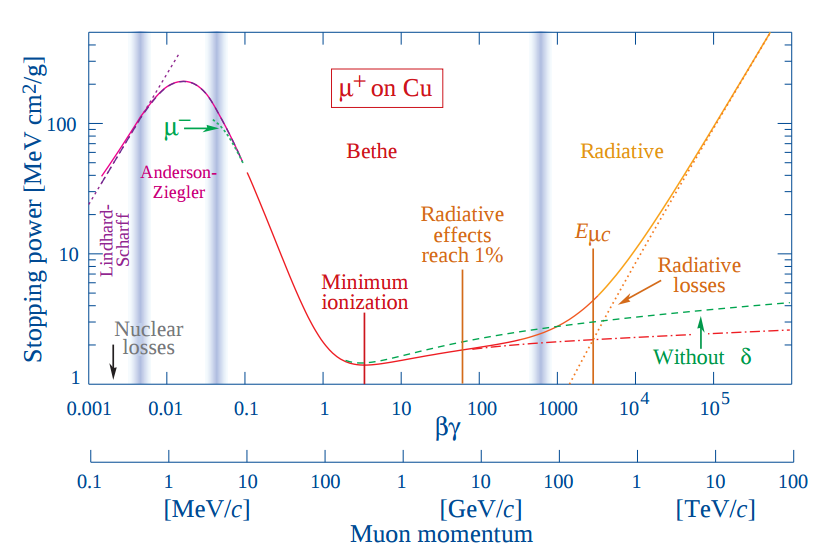
\includegraphics[width=0.95\textwidth]{bethe}
	\caption{Stopping power for positive muons in copper as a function of $\beta\gamma$. The solid curves show the total stopping power. The vertical lines show the range of validity of the curves \cite{pdg}.}
	\label{pbethe}
\end{figure}\no
This equation is valid in the energy range from $6\,$MeV up to $6\,$GeV or more generally $0.02 < \beta < 0.99$ within $1\,$\% accuracy. Below that limit the processes can be described by solid state physics and for higher energy Bremsstrahlung becomes dominant. The formula is completely independent of the mass of the traversing particle, the stopping power only depends on its speed and charge. By dividing by the density it becomes also almost independent of the target material. These facts demonstrate the universality of the equation.\\
In between the limits of the validity there are three prominent regions. For small $\beta\gamma$ the energy loss follows approximately $1/\beta^2$ until it reaches a broad minimum for $\beta\gamma \cong 3.5 $. A particle in this region is called \ac{MIP}. For larger $\beta\gamma$ the energy loss starts increasing again in a region referred to as logarithmic (or relativistic) rise.\\
Though not depending on the mass, the interacting particles still have to be a couple of orders of magnitude heavier than the electrons they are interacting with. That is why this formula does not apply to electrons or positron as incident particles. Their behaviour is shown in \ar{pelec}. For low energies the energy losses is mostly due to ionisation. For the most materials Bremsstrahlung becomes dominating above a critical energy of a few tens of MeV. A comparison between Bethe-Bloch and the stopping power for electrons is shown in \ar{pbetheall}.
\begin{figure}[ht]
	\centering
	\subbottom[Energy loss in lead as a function of electron or positron energy \cite{pdg}.]{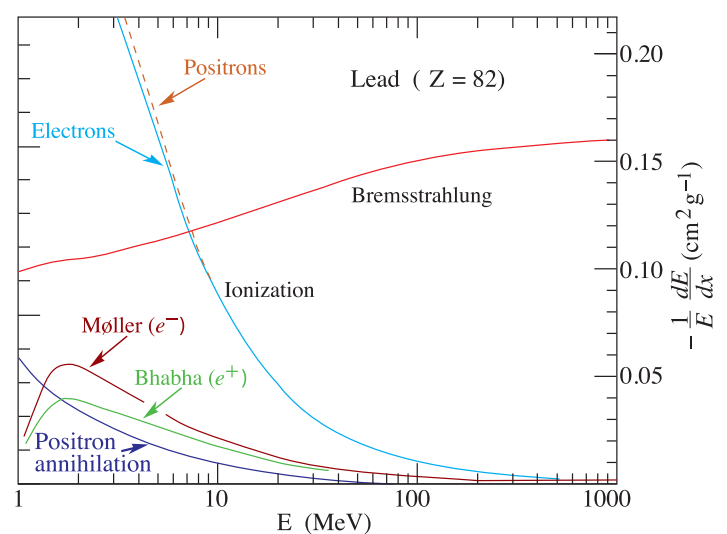
\includegraphics[width=0.47\textwidth]{elec}\label{pelec}}
	\hfill
	\subbottom[Energy loss for several positive particles in carbon \cite{murphy}.]{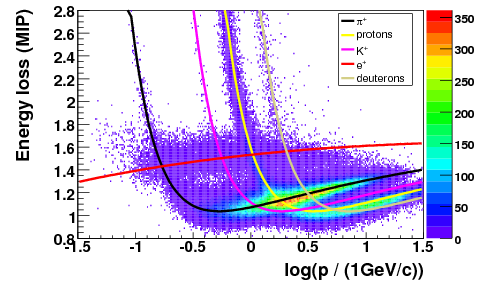
\includegraphics[width=0.47\textwidth]{betheall}\label{pbetheall}}
	\caption{Comparison of the stopping power of electrons/positrons and heavier charged particles.}
	\label{pcomp}
\end{figure}\no
% ========================================================
\subsection{Energy Loss Distribution}\label{slandau}
The Bethe-Bloch formula only describes the mean energy loss of a particle passing through matter. Since this is a statistical process the single values follow a certain distribution. For the material thickness of all utilised detectors during this thesis they follow a highly-skewed Landau (or Landau-Vavilov) distribution as shown in \ar{plan1}. If the thickness is increased the distribution gets less skewed as demonstrated in \ar{plan2} \cite{pdg}.
\begin{figure}[ht]
	\centering
	\subbottom[Electronic energy deposition distribution for a $10\,$GeV muon traversing $1.7\,$mm of silicon. $M0(\Delta)$ and $M1(\Delta)$ are the cumulative 0th moment (mean number of collisions) and 1st moment (mean energy loss) in crossing the silicon \cite{pdg}.\label{plan1}]{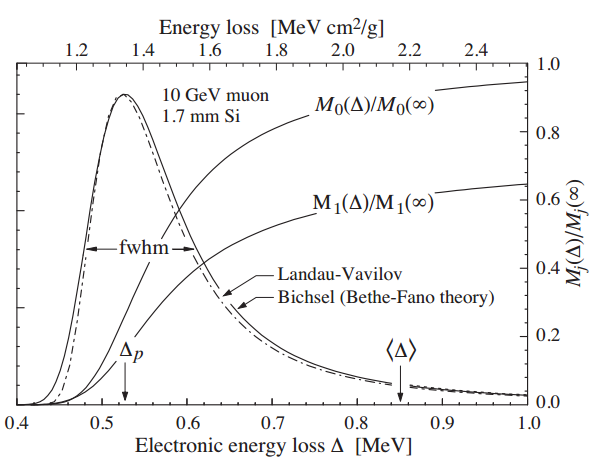
\includegraphics[width=0.47\textwidth]{landau1}}
	\hfill
	\subbottom[Normalised Straggling functions in silicon for $500\,$MeV pions. $w$ is the full width at half maximum \cite{pdg}.\label{plan2}]{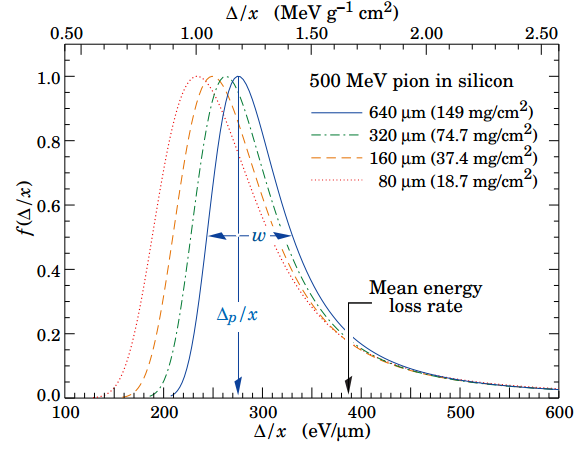
\includegraphics[width=0.47\textwidth]{landau2}}
	\caption{Distribution of the energy loss.}
	\label{plan}
\end{figure}\no
% ========================================================
% SEMICONDUCTOR DETECTORS
% ========================================================
\section{Semiconductor Detectors}
Semiconductor detectors are extensively used in particle physics to detect ionising particles. For the detectors used in this thesis it is important to get information about the spatial position of a particle and the amount of electrons created in the material. The most widely used semiconductor is silicon, which is also the material of the current tracking detector at \ac{CMS}. There are generally two different types of silicon tracker detectors: pixel and strip detectors, of which the former has a two dimensional and the latter has a one dimensional resolution. Using several layers of pixel or intersecting strip detectors (or a combination of both) achieves three dimensional reconstruction.\\
The working principle of a semiconductor detector is summarised in the following.
% ========================================================
\subsection{Semiconductor Basics}
A semiconductor is a material with an electric conductivity that lies between a conductor and an insulator. Responsible for that behaviour is their unique band structure, which is shown in \ar{pband}. The shell structure of the atoms in a bulk material consists of continuous energy bands of which two are responsible for the electric conductivity of the material: The highest band (in energy) that is completely occupied, the valence band, and the next highest band called conduction band. If an electron is lifted from the valence band to the conduction band, two charge carriers are created: the ``free'' electron in the conduction band and the electron ``hole'' in the valence band, which are called together an electron-hole pair.\\
Semiconductors are defined by the energy difference of the two bands that is called band gap energy. Semiconductors have band gaps that are smaller than about $4\,$eV and larger than $0.4\,$eV. A band gap of $0\,$eV would correspond to a metal and one above $4\,$eV to an insulator. This is the very behaviour that is exploited for particle detectors. If a particle traverses a semiconductor it looses energy due to ionisation as shown in \ar{sbethe} and thereby creates electron-hole pairs.
\begin{figure}[ht]
	\centering
	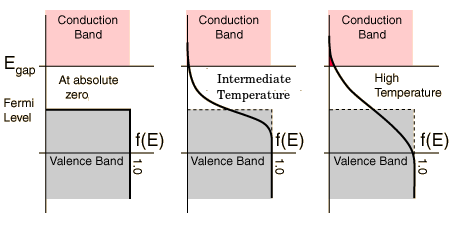
\includegraphics[width=0.6\textwidth]{band}
	\caption{Simplified band structure for a semiconductor at different temperatures. $f(E)$ denotes the Fermi distribution of the electron of the valence band. At temperatures above zero some electrons of the valence band have enough thermal energy to be lifted into the conduction band \cite{hyperphys}.}
	\label{pband}
\end{figure}\no
% ========================================================
\subsection{Signal to Noise}
As demonstrated in \ar{pband} the conductivity of semiconductors is temperature dependent due to the Fermi distributed electrons. Most semiconductors are already conductive at room temperature because some electrons have enough thermal energy to overcome the band gap. Using the Fermi distribution:
\begin{equation}
	f(E) = \frac{1}{1+e^{\frac{E-E_{f}}{kT} }}
\end{equation}
where $E_{f}$ refers to the Fermi energy, $T$ to the temperature and $k$ to the Boltzmann constant, the mean number of thermally created electron-hole pairs is about $3900$ per cubic millimetre at room temperature. Reading of \ar{plan2} the mean loss of energy for a \ac{MIP} is $1.65\,$MeV\,cm$^{2}$/g which corresponds for silicon with a density of $2.33\,$g/cm$^{3}$ to $3.84\,$MeV/cm. The average energy to produce an electron-hole pair is about $3.6\,$eV. Hence, the mean energy a \ac{MIP} loses in a silicon bulk with a thickness of $285\,\upmu$m equates to $30500$ electron-hole pairs. From this it follows that the thermal noise of a $12\,$cm strip detector of \ac{CMS} is of the same order of magnitude as the signal. For a \ac{CMS} pixel it is still around $5\,$\% of the signal. In order to conduct precise measurements, it is important to reduce the signal to noise ratio.
% ========================================================
\subsection{Doping \& pn-junction}
To overcome the free charge carriers at room temperature a reversed biased pn-junction is used, that fully depletes the silicon bulk.\\
All pure element semiconductors come from the carbon group because they have exactly four valence electrons and can either lose or gain electrons at the same time. There are two types of doping:
\begin{description}
	\item[n-type:]{Doping with elements from the nitrogen group (donor atoms, e.g. Arsenide or Phosphor) leads to an excess of loosely bound electrons in the lattice which shifts the Fermi energy closer to the conduction band.}
	\item[p-type:] Doping with elements from the boron group (acceptor atoms, e.g. Boron) leads to an excess of loosely bound holes in the lattice which shifts the Fermi energy closer to the valence band.
\end{description}
A pn-junction is created by bringing n-doped and p-doped semiconductors in contact with each other, which will cause a density gradient of the majority charge carriers across the junction. The electrons and holes wills diffuse into the opposite doped material and recombine to from a depletion zone with no free charge carriers. This results in a net movement of the electric charge and builds up an electric field across the junction until an equilibrium is established between diffusion and Coulomb force. 
% ========================================================
\subsection{Operation Mode}
If an external voltage is applied with the same polarity as the intrinsic potential barrier the depletion zone will increase; this is the process referred to as reverse biasing. In that way it is possible to deplete the whole bulk form charge carriers. Semiconductor detectors are usually operated over-depleted to be certain to create an electric field across the full detector volume. When a charged particle creates electron-hole pairs in that state, the charge carriers will drift to either side of the semiconductor parallel to the electric field and induce signals at the electrodes.\\
These are the very signals that are sent to the \ac{ROC} of the \ac{CMS} pixel detector (q.v. \ar{s130}) in order to detect these particles.
% ========================================================
% SCINTILLATORS
% ========================================================
\section{Scintillation Detectors}
\begin{figure}[ht]
	\centering
	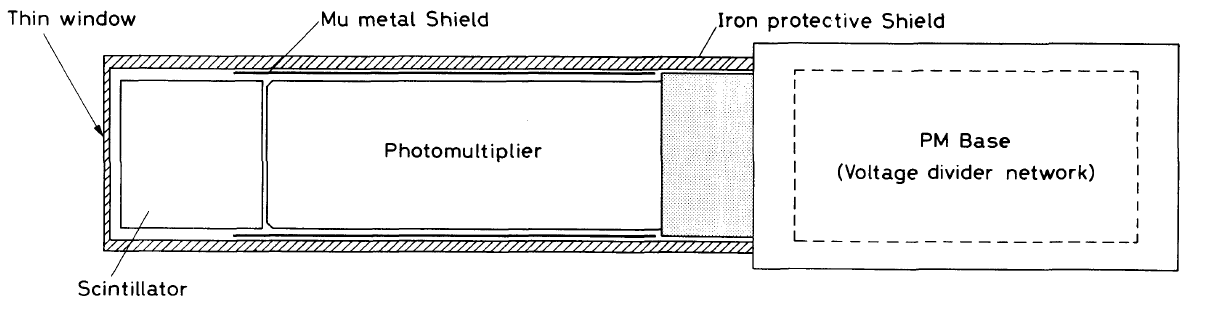
\includegraphics[width=0.94\textwidth]{scint}
	\caption{Schematic composition of a scintillation detector \cite{leo}.}
	\label{pscint}
\end{figure}\no
Scintillators belong to the most often and widely used particle detections devices in nuclear and particle physics. They make use of the property that some materials emit a short flash of light when hit by a nuclear particle or radiation. In the following the working principle of a scintillator will be sketched, for more information see \cite{leo}.\\
\ar{pscint} shows the basic elements of a scintillation detector. In general, it consists of a scintillating material that is optically coupled to a \ac{PM}, which either happens directly or via a light guide. Radiation or particles passing through the scintillator excite molecules and/or atoms which then causes the material to emit light. The light is guided to the the \ac{PM} where it is converted into a current by utilising the photoelectric effect. Thereupon the current is amplified by an electron multiplier, s.t. it is large enough to be measured. Depending on the material, scintillators provide some very useful features, e.g.:
\begin{itemize}
	\item sensitivity to the deposited energy
	\item fast time responses
	\item pulse shape discrimination (allows for particle identification)
\end{itemize}
Scintillation detectors exploit the so-called luminescence, which is the property to absorb incoming energy and re-emit it as light. If the re-emission happens within $10\,$ns, luminescence is called fluorescence. If it takes longer it is called phosphorescence. For scintillators only fluorescence serves. The time evolution of the re-emission follows an exponential decay of the excited states, which is split into two components as shown in \ar{pdecay}.\\
A viable scintillation detector has to meet the following requirements:
\begin{enumerate}
	\item a high conversion efficiency.
	\item transparency to the self emitted light.
	\item light emission in the spectral range of the \ac{PM}.
	\item a short decay constant.
\end{enumerate}
There are six different types of scintillating materials that split into organic and inorganic ) materials. The organic materials are either crystals, liquids or plastic and the inorganic materials are either crystals, gases or glasses.
\begin{figure}[ht]
	\centering
	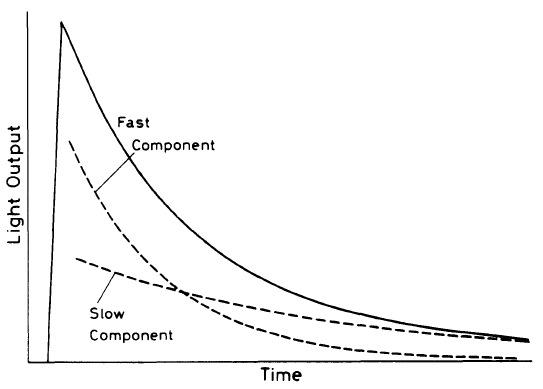
\includegraphics[width=0.5\textwidth]{decay}
	\caption{Exponential decay of fluorescent radiation with a prompt and a delayed component. The solid line corresponds to the total decay. \cite{leo}.}
	\label{pdecay}
\end{figure}\no
% ========================================================
% \subsection*{Plastic Scintillators}
% Plastic Scintillators are probably the most widely used organic detectors
% \begin{wrapfigure}{r}{4.5cm}
% 	\vspace*{-5pt}
% 	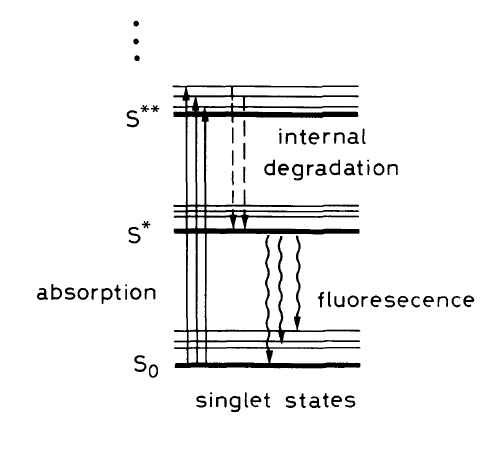
\includegraphics[width=4.4cm]{pimol}
% 	\caption{Energy level diagram of an organic scintillator molecule \cite{leo}}
% 	\label{ppimol}
% 	\vspace*{-5pt}
% \end{wrapfigure} 
% in particle physics due to their extremely fast signals of $2-3\,$ns and their good flexibility. They are a solution of organic scintillators in a solid plastic solvent like polyvinyl toluene, polyphenylbenzene or polystyrene. The solutions themselves are aromatic hydrocarbon compounds with a linked or condensed benzene ring structure. A typical example of an organic scintillator material is shown in \ar{ppbd}.\\
% The light in organic materials is produced by a transition of free valence electrons of the molecules where the delocalised electrons occupy $\uppi$-molecular orbits. An exemplary energy level diagram of that process is shown in \ar{ppimol}, where the ground state is singlet state $S_{0}$ with two excited electronic states $S^{*}$ and $S^{**}$ above. Each of the states has a fine structure due to vibrational modes. Penetrating radiation and particles excite both electron and vibrational levels (solid arrows) which generally decay immediately to $S^{*}$ (dashed arrows) without emission of light. $S^{*}$ in turn has a high probability to decay radiatively to one of the vibrational states of $S_{0}$ (waved arrows).This is causing the prompt component of the fluorescence, the delayed component originates from a triplet state with similar properties. The fact that $S^{*}$ decays to excited vibrational states of $S_{0}$ with a radiation energy less than $S_{0}$ $\rightarrow$ $S^{*}$ allows for the transparency to the own emitted light.\\
% \begin{figure}[ht]
% 	\centering
% 	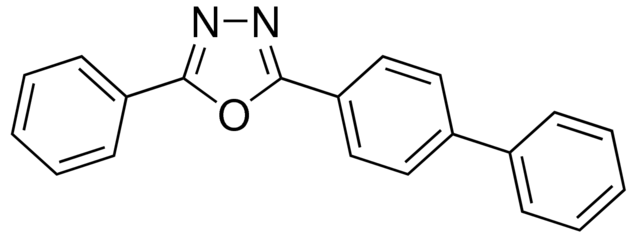
\includegraphics[width=0.5\textwidth]{pbd.png}
% 	\caption{2-(4-Biphenylyl)-5-phenyl-1,3,4-oxadiazole (PBD), \protect\chemfig{C_{20}H_{14}N_2O}.}
% 	\label{ppbd}
% \end{figure}\no
% ========================================================
% ELECTRONICS
% ========================================================
\section{Electronics}
In order to deliver the signals, to transform them or to build a trigger logic a lot electronics is required. Explaining every single device, which was used would go rather too far. Nevertheless it is quite important to possess knowledge about the two electronic standards NIM and \ac{TTL}.
% ========================================================
\subsection{NIM}
\begin{figure}[ht]
	\centering
	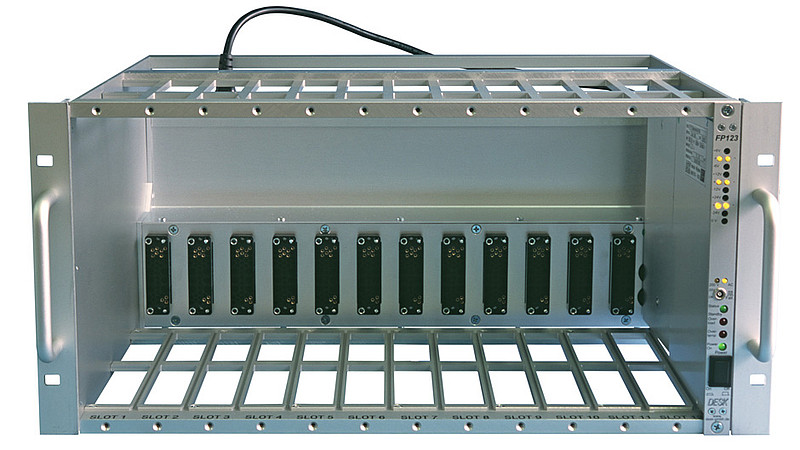
\includegraphics[width=0.95\textwidth]{nim}
	\caption{A standard NIM bin}
	\label{pnim}
\end{figure}\no
Initially NIM was an acronym for Nuclear Instrument Modules. However, as the use and manufacture spread farther throughout the world and it became truly international they were still identified with NIM. Having a company name as acronym was not appropriate any more and attempts to fit suitable words to the initials were in vain. So nowadays NIM only stands for NIM.\\
NIM is modular system and was the first and simplest standard established in particle physics. All basic apparatus, e.g. amplifiers, discriminators or scalers were designed in standard mechanical and electrical specifications. They fit into standardised so-called \textit{bins} that deliver the supply voltage via a rear plug of the device. Thereby it is very easy to build specific electronic system with many devices, like a trigger logic for example. They have an enormous flexibility.\\
The standard modules are $3.43\,$cm wide and have height of $22.2\,$cm  which also allows for multiples of that standard, i.e. double-width, triple-width, etc. A standard NIM fits $12$ single modules and is shown in \ar{pnim}.
% ========================================================
\subsection*{NIM Signals}
NIM include devices with both analogue and digital signals. The digital or logic signals have a fixed shape and only know the two states ON and OFF or equivalently 1 and 0.\\
There exist two types of standards called slow-positive and fast-negative. The latter one is referred to as NIM logic and has extremely fast rise times of the order of a nanosecond and a comparable width. The NIM logic levels are defined in \ar{tnim}. This definition is current based and all the input and output impedances are required to be $50\,\Upomega$. Fast-negative signal may be transported through long cables.
\begin{table}[ht]
	\centering
	\begin{tabular}{c|r c r|r c r!{\vrule width 2pt}r}
		\noalign{\hrule height 2pt}
				& \multicolumn{3}{c|}{\textbf{Output must deliver}} 	& \multicolumn{3}{c!{\vrule width 2pt}}{\textbf{Input must accept}} & \textbf{Voltage}							\\\hline
		Logic 1 & $-14\,$mA	&to	& $-18\,$mA							& $-12\,$mA	&to	& $-36\,$mA		& \multicolumn{1}{r}{$-0.8\,$V}	\\	
		Logic 0 & $-1\,$mA  &to	& $1\,$mA							& $-4\,$mA	&to	& $20\,$mA		& \multicolumn{1}{r}{$0\,$V}	\\
		\noalign{\hrule height 2pt}
	\end{tabular}
	\caption{Fast negative NIM logic. Neither rise time nor width are defined \cite{leo}.}
	\label{tnim}
\end{table}
% ========================================================
\subsection{\ac{TTL} Signals}
\ac{TTL} is no part of the NIM standard even though it is often used in particle physics. That is why this positive going logic is often found in NIM modules. Its levels are voltage based and can be found in \ar{tttl}.
\begin{table}[ht]
	\centering
	\begin{tabular}{c|r c r|r c r}
		\noalign{\hrule height 2pt}
				&  \multicolumn{3}{c|}{\textbf{Voltage}}							&  \multicolumn{3}{c}{\textbf{Corresp. current}}	\\\hline
		Logic 1	& $2\,$V	& $-$	& $5\,$V							& $40\,$mA	& $-$	& $100\,$mA				\\	
		Logic 0 & $0\,$V  	& $-$	& $0.8\,$V							& $0\,$mA	& $-$	& $16\,$mA				\\
		\noalign{\hrule height 2pt}
	\end{tabular}
	\caption{TTL signal levels \cite{leo}.}
	\label{tttl}
\end{table}
% ========================================================
